% \documentclass[12pt,titlepage]{article}
% 
% %% THE USEPACKAGES NECESSARY FOR THIS EXAMPLE
% %% NOTE THAT genetics_manu_style MUST BE CALLED AFTER mychicago
% \usepackage{graphicx}
% %\usepackage{figcaps}
% \usepackage[nomarkers,notablist,nofiglist,tablesfirst]{endfloat}
% \usepackage{amsfonts}
% \usepackage{sectsty}
% %\usepackage{subfigure}
% %\usepackage{subcaption}
% \usepackage{natbib} \bibpunct{(}{)}{;}{author-year}{}{,} 
% \usepackage[usenames,dvipsnames,svgnames,table]{xcolor}
% %\allsectionsfont{\sffamily}
% %% THE MANUSCRIPT TITLE
% 
% \usepackage{caption}
% \usepackage[labelformat=simple]{subcaption}
% 
% \usepackage{bibentry}
% 
% \usepackage{xr}
% \externaldocument{hybrid_zone}
% 
% \newcommand{\alisa}[1]{{\em \color{red} #1}}
% \newcommand{\plr}[1]{{\em \color{blue} #1}}
% \newcommand{\yb}[1]{{\em \color{magenta} #1}}
% 
% 
% \newcommand{\given}{\,\vert\,}
% \newcommand{\st}{\,\colon\,}
% \renewcommand{\and}{\,\&\,}
% 
% 
% \begin{document}
\setcounter{table}{0}
\renewcommand{\thetable}{S\arabic{table}}
\setcounter{figure}{0}
\renewcommand{\thefigure}{S\arabic{figure}}

\begin{figure}
    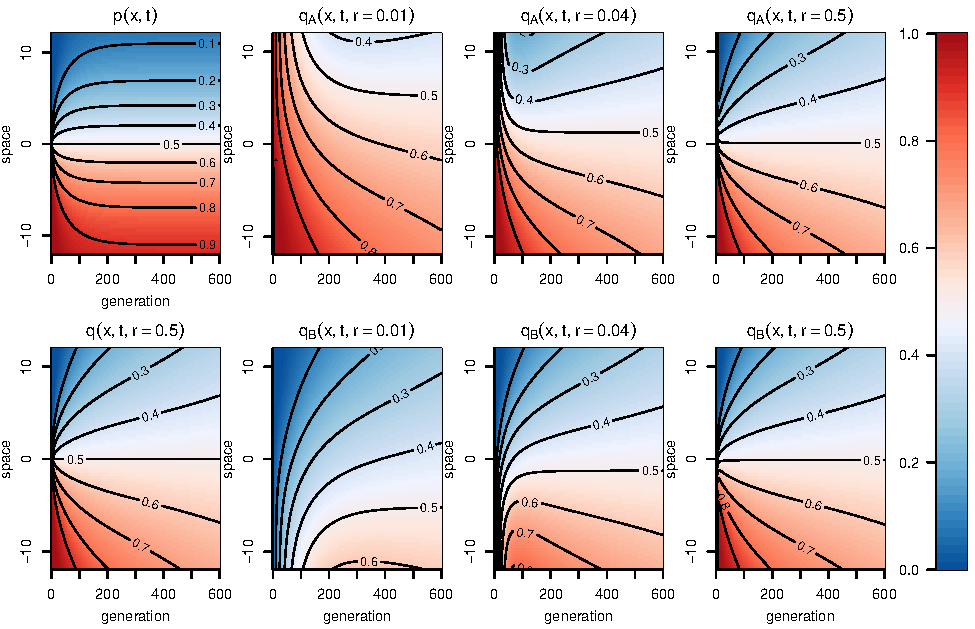
\includegraphics{figs/linked-frequencies-longtime.pdf}
    \caption{
        \textbf{Probabilities of $A$ ancestry,}
        across space (vertical axis, in units of $\sigma$) 
        and time (horizontal axis, in generations).
        In each plot, color corresponds to the expected frequency of $A$ ancestry
        at a particular location in time and space.
        The selection coefficient is $s=.02$.
        \textbf{Top left:} at the selected site, showing establishment and stabilization of the cline
        on a time scale of $1/s=50$ generations.
        \textbf{Bottom left:} at an unliked site,
        with cline flattening continuing with $\sqrt{t}$.
        Remaining figures show frequencies of $A$ ancestry \emph{conditional}
        on the ancestry at the selected site,
        at different distances from the selected site ($r=.01$, .04, and 0.5 Morgans),
        as described in the text (see definition of $q_z(x,t,r)$).
        See figure \ref{fig:linked_cline_heatmaps}
        for the same figure over a shorter period of time.
    }
    \label{sfig:linked_cline_heatmaps_longtime}
\end{figure}




\begin{figure}
    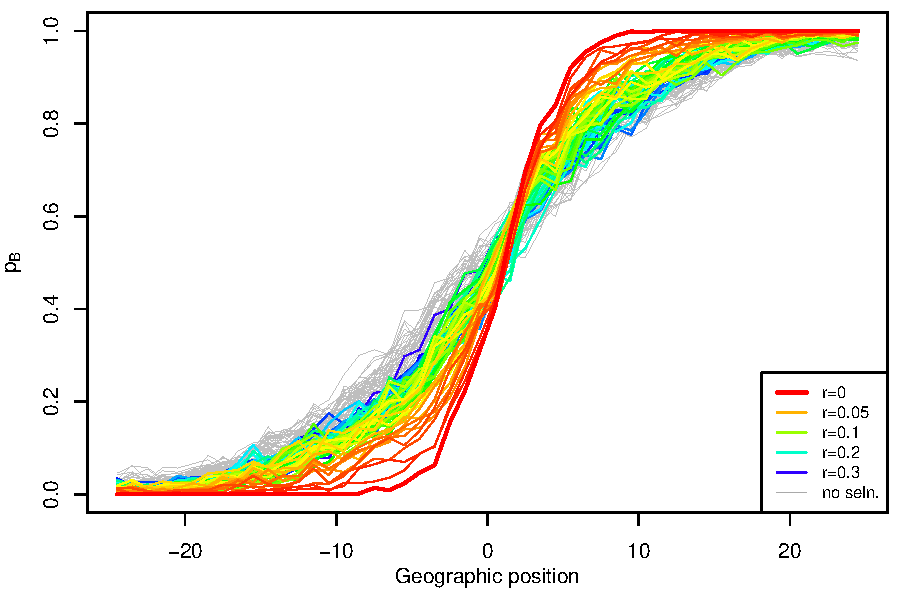
\includegraphics{figs/alleleFrequencies_sim.pdf}
    \caption{
    Frequency of ancestry $B$,
    across geography at different physical positions on the genome, simulated for a hybrid zone
     $T=100$ generations after secondary contact, with $s=0.1$,
     using 50 demes, each with 500 diploid individuals and $\sigma=1$.
    Each line represents a locus some distance $r$ away from the true target of selection.
    Grey lines represent the same positions from a simulation with
    identical parameters except that $s=0$.
    Corresponding theoretical quantities are shown juxtaposed in Figure \ref{sfig:alleleFreq_tau100_comparison};
    the same plot is shown with weaker selection in Figure \ref{alleleFreq_tau100_weaker_s} and at a longer time in Figure \ref{alleleFreq_tau1000}.
}\label{alleleFreq_tau100}
\end{figure}



\begin{figure}
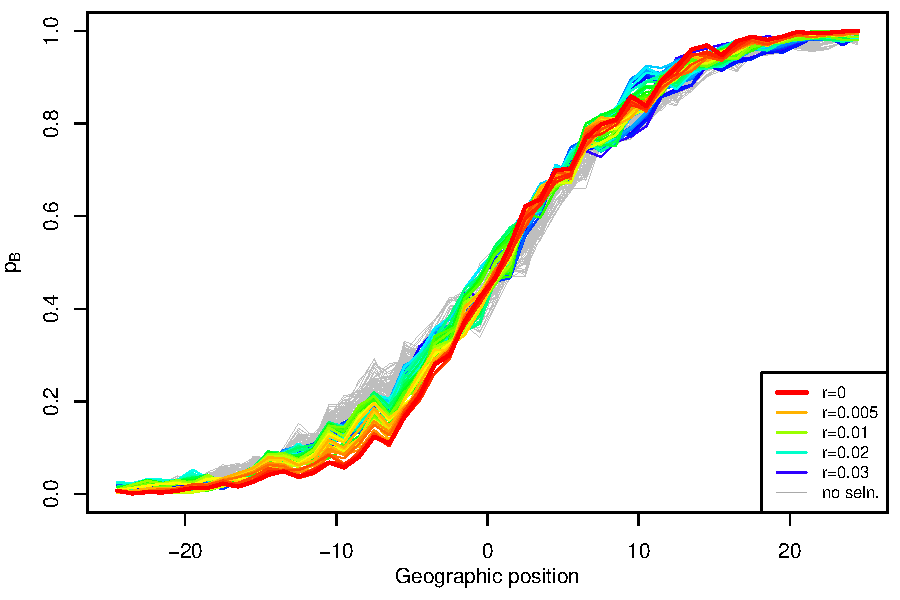
\includegraphics{figs/alleleFrequencies_sim_s01_tau100_closely_linked.pdf}
\caption{
    Frequency of ancestry $B$,
    across geography and at several physical positions on the genome, simulated for a hybrid zone
     $T=100$ generations after secondary contact,
    and with $s=0.01$.
        50 demes, each with a population size of 500 diploid individuals.
    Each line represents a locus some distance $r$ away from the true target of selection, 
    and $r=0$ represents the locus that is under selection. Grey lines represent the same positions from a simulation with
    identical parameters except that $s=0$.
}\label{alleleFreq_tau100_weaker_s}
\end{figure}

\begin{figure}
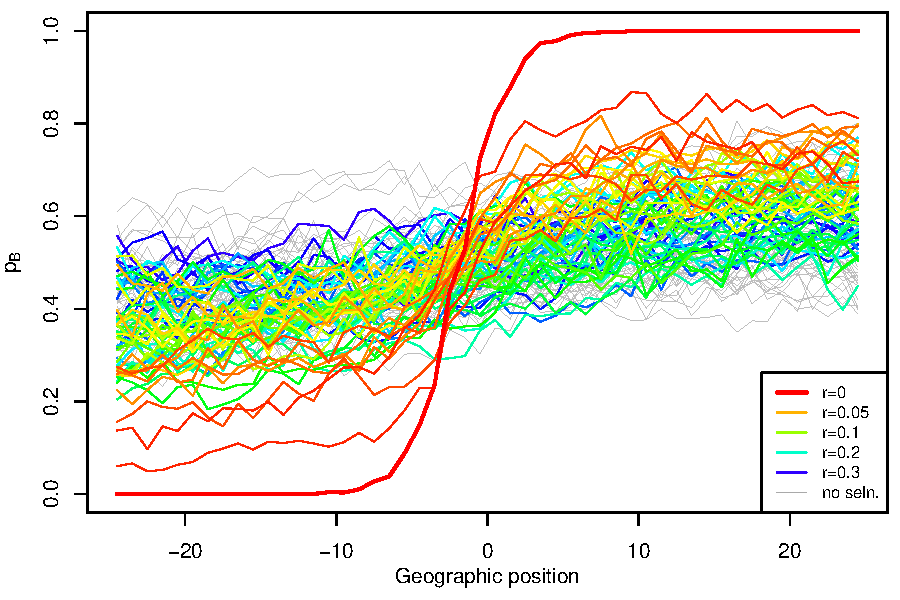
\includegraphics{figs/alleleFrequencies_sim_s1_tau1000.pdf}
\caption{
    Frequency of ancestry $B$,
    across geography and at several physical positions on the genome, simulated for a hybrid zone
     $T=1000$ generations after secondary contact,
    and with $s=0.1$.
        50 demes, each with a population size of 500 diploid individuals.
    Each line represents a locus some distance $r$ away from the true target of selection, 
    and $r=0$ represents the locus that is under selection. Grey lines represent the same positions from a simulation with
    identical parameters except that $s=0$.
 }\label{alleleFreq_tau1000}
\end{figure}



\begin{figure}
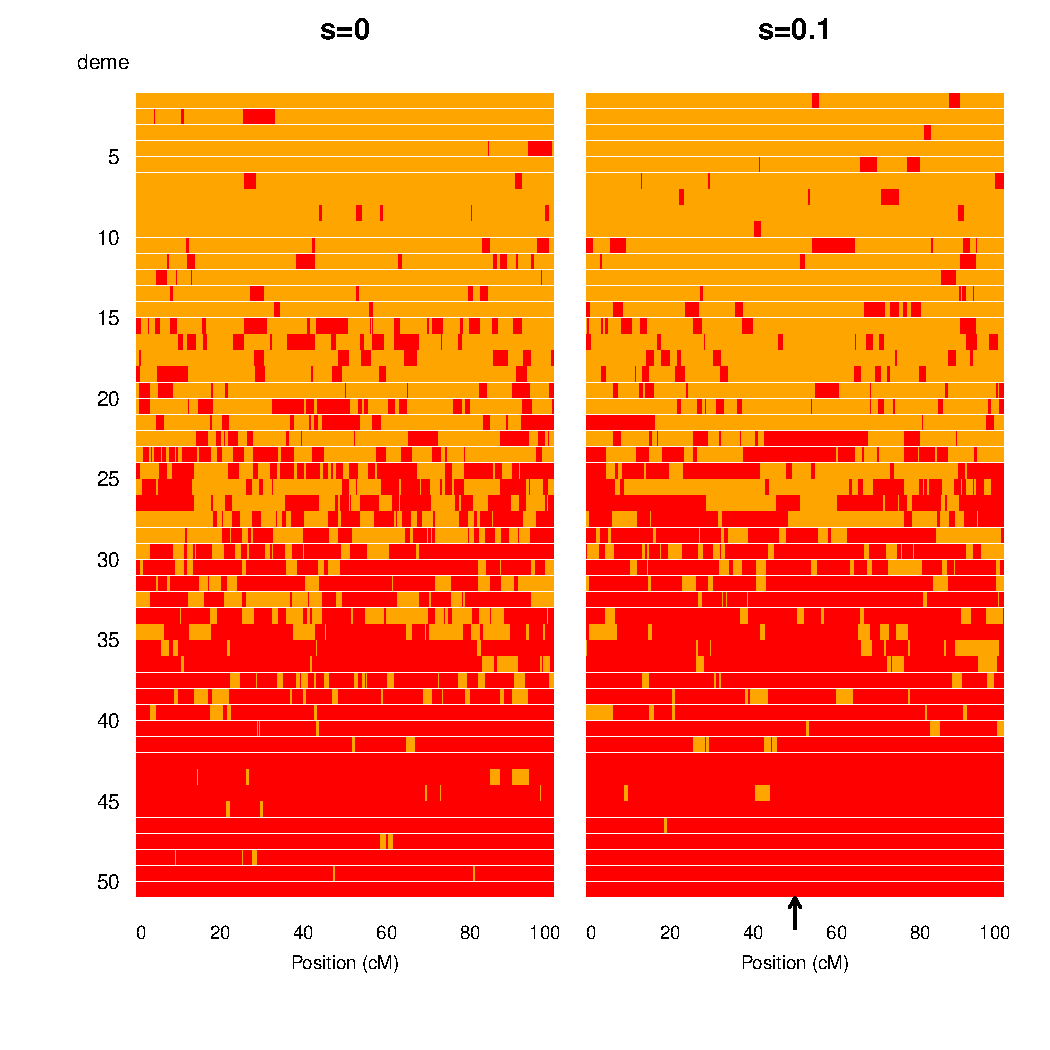
\includegraphics[width=\textwidth]{figs/plot_chromosomes_tau100.pdf}
\caption{Randomly sampled chromosomes  across a hybrid zone of age $T=100$. Here we compare chromosomes of length 1M from a neutral zone to one that has a single under-dominant locus ($s=0.1$) in the middle of the chromosome (indicated by black arrow). Red blocks along the chromosome denote ancestry $B$, and orange blocks are ancestry $A$.
 }\label{Fig:resistanceToIntrogression100g}
\end{figure}


\begin{figure}
    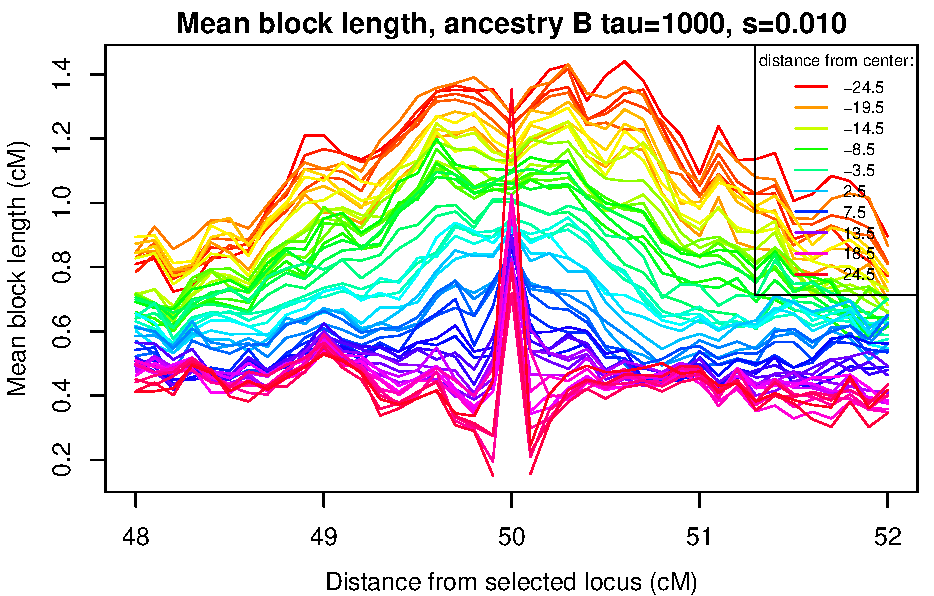
\includegraphics{{figs/simulation_SIGMA1_Ninds25000_ndemes50_s0.01_tau1000_blocksAlongChromAncBConditioning_nonnormalized}.pdf}
    \caption{
        \textbf{Mean haplotype lengths of $B$ haplotypes}, $l_B(x,m)$,
        across the genome (horizontal axis) and at differntial spatial locations (colored lines),
        from a simulation with 50 demes having 500 individuals each, $s=0.01$, $\sigma=1$, and after $T=1000$ generations.
    } \label{sfig:blocksAlongChromAncBConditioning_nonnormalized}
\end{figure}

\begin{figure}
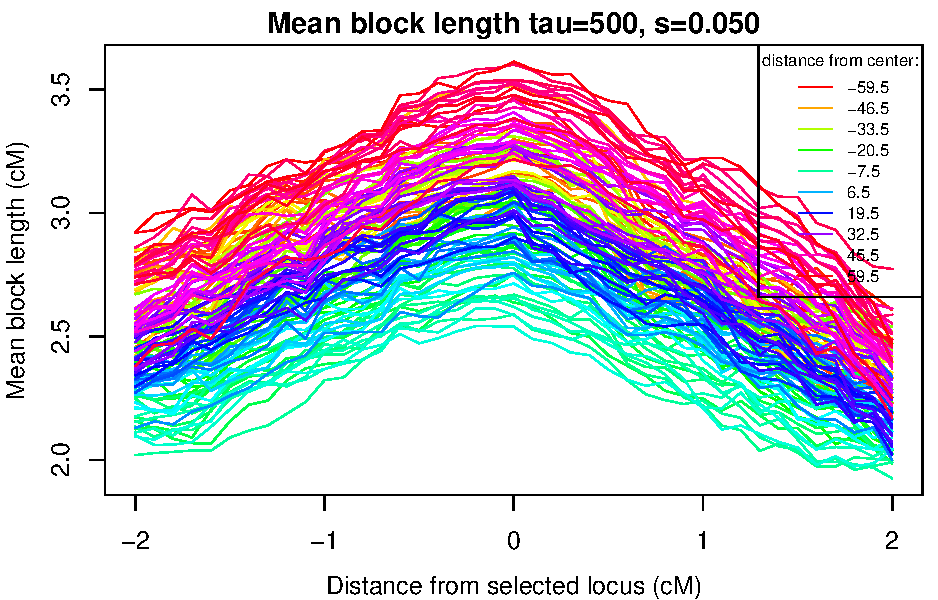
\includegraphics[width=\textwidth]{{figs/results_runid_753324_chr1_start0.48_stop0.52_by0.001_blocksAlongChromNoConditioning_nonnormalized}.pdf}
\caption{
    \textbf{Mean enclosing block length $l(m,x)$}, across the genome (horizontal axis)
    and at different geographic positions (different colored lines).
    Results are from a simulation with 120 demes of 200 diploids each, selection $s=.05$, dispersal $\sigma=3$, 
    and after $T=500$ generations.
}\label{Fig:meanBlockLengthsUnconditioned}
\end{figure}


\begin{figure}
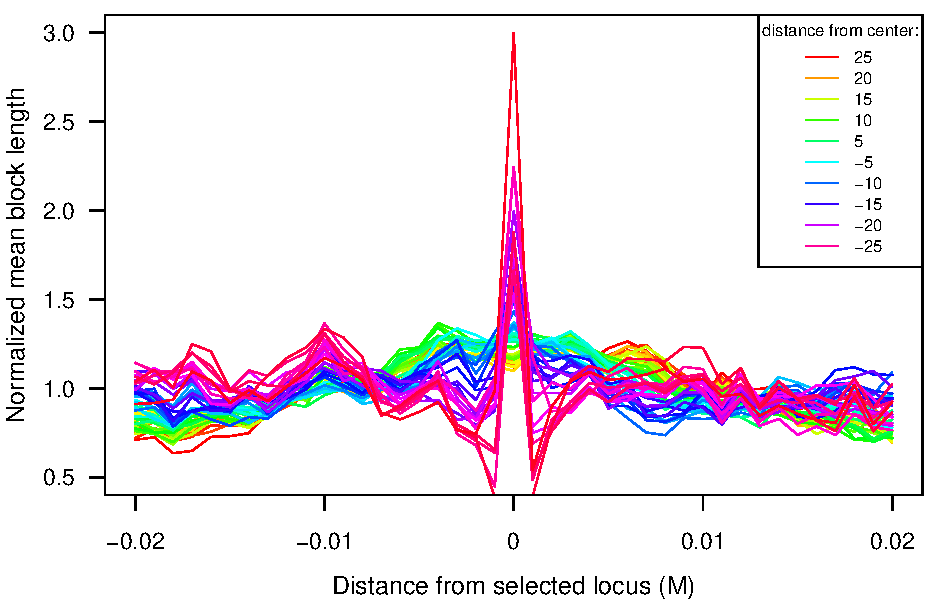
\includegraphics{figs/blocksAlongChromAncBConditioning.pdf}
\caption{
    \textbf{Normalized mean enclosing block length}, $l_B(m,x)$, after $T=1000$ generations,
    against position relative to the selected locus (horizontal axis)
    located in the center of a 1M chromosome.
    Each line shows the mean block length at that spatial and genomic position
    divided by the mean over the chromosome at that location;
    the simulation was run with $s=1$ and $\sigma=1$,
    50 demes, each containing 500 diploid individuals.
}\label{Fig:blockLengths}
\end{figure}


\begin{figure}
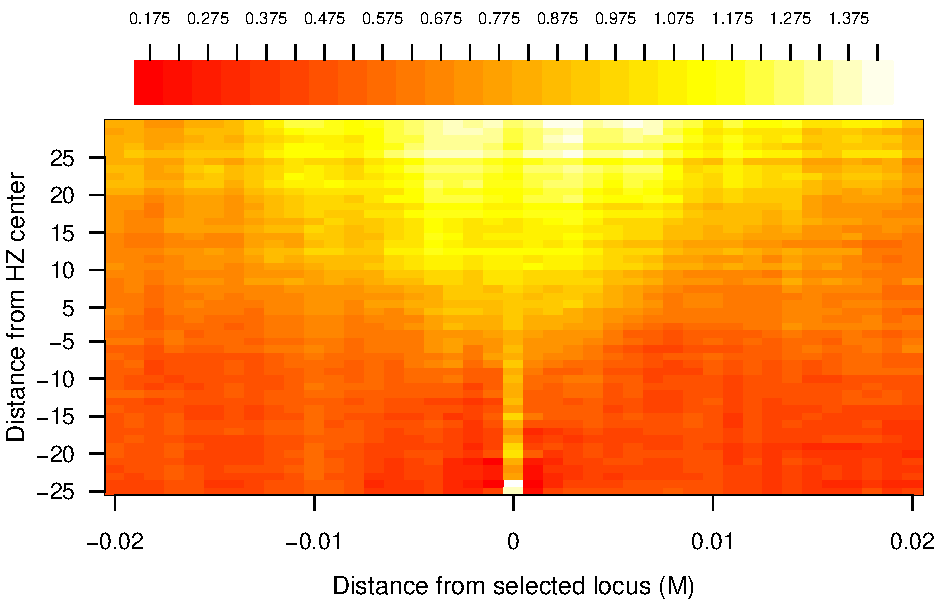
\includegraphics{figs/blocksAlongChromHeatmapAncBConditioning.pdf}
\caption{Heatmap of mean block length $l_B(m)$ along a simulated chromosome. }\label{Supp:blockLengthHeatmap}
\end{figure}




\begin{figure}
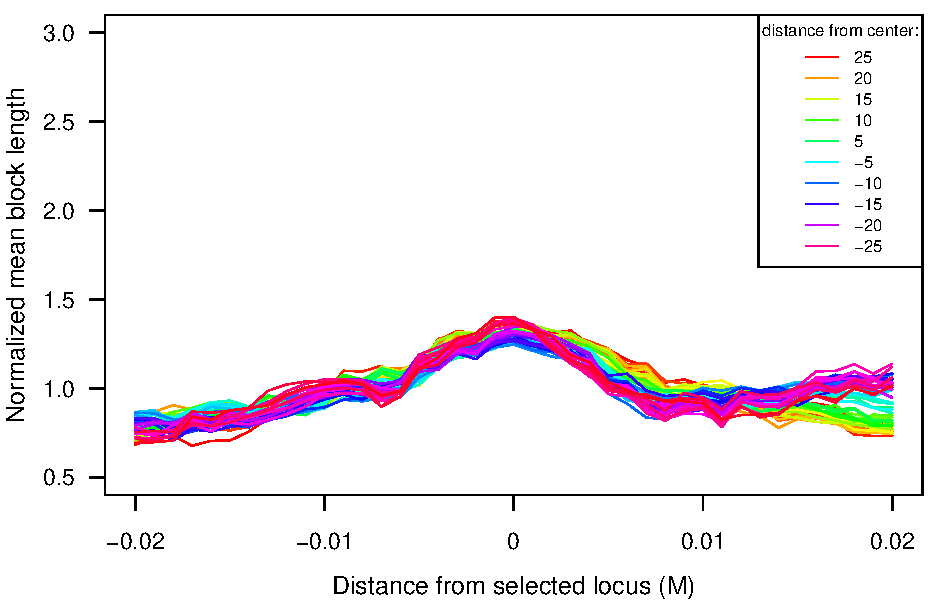
\includegraphics{figs/blocksAlongChromNoConditioning.pdf}
\caption{Heatmap of mean block length $l(m)$ surrounding a given position along the genome with a single underdominant site ($s=0.01, T=1000$). }\label{Supp:blockLengthNoAnc}
\end{figure}

\begin{figure}
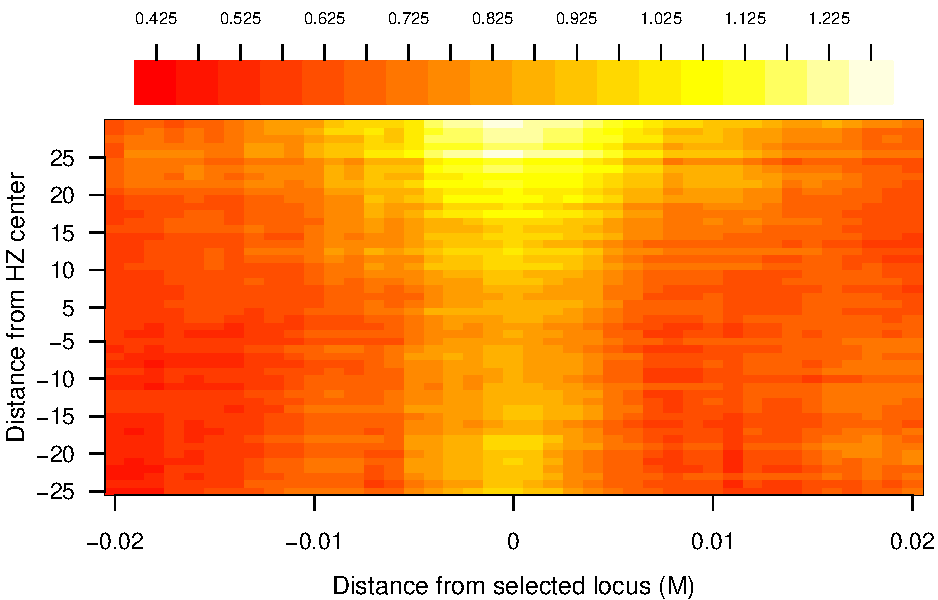
\includegraphics{figs/blocksAlongChromHeatmap.pdf}
\caption{Heatmap of mean block length $l(m)$ along a simulated chromosome with a single underdominant site ($s=0.01, T=1000$) }\label{Supp:blockLengthHeatmapNoAnc}
\end{figure}


\begin{figure}
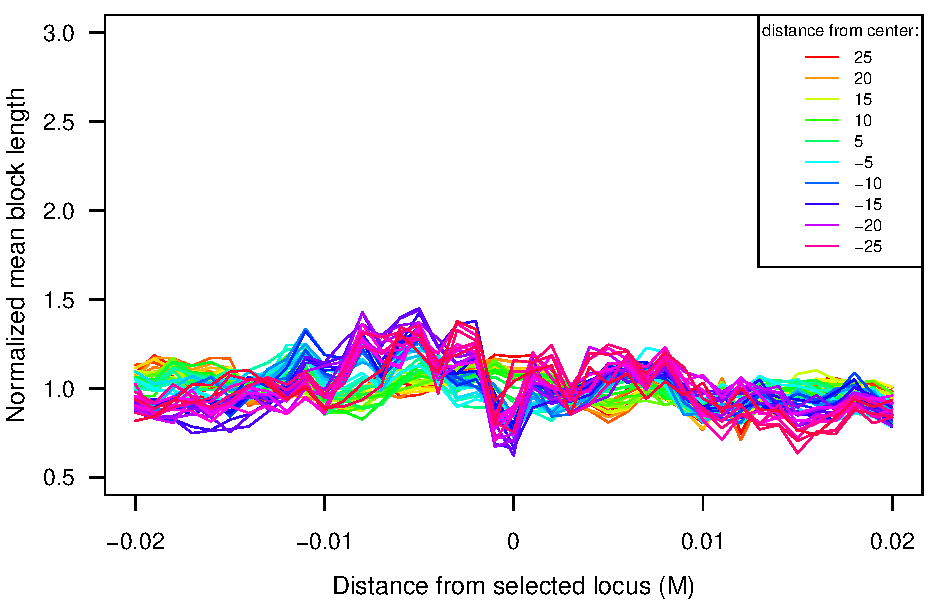
\includegraphics{figs/adjacentBlocksAlongChromAncBConditioning.pdf}
\caption{Mean block length of $l_A(m\pm)$ across chromosome with single under dominant site, conditioning on ancestry $B$ at the selected locus. ($s=0.01, T=1000$)}\label{Supp:adjacentBlocks}
\end{figure}


\begin{figure}
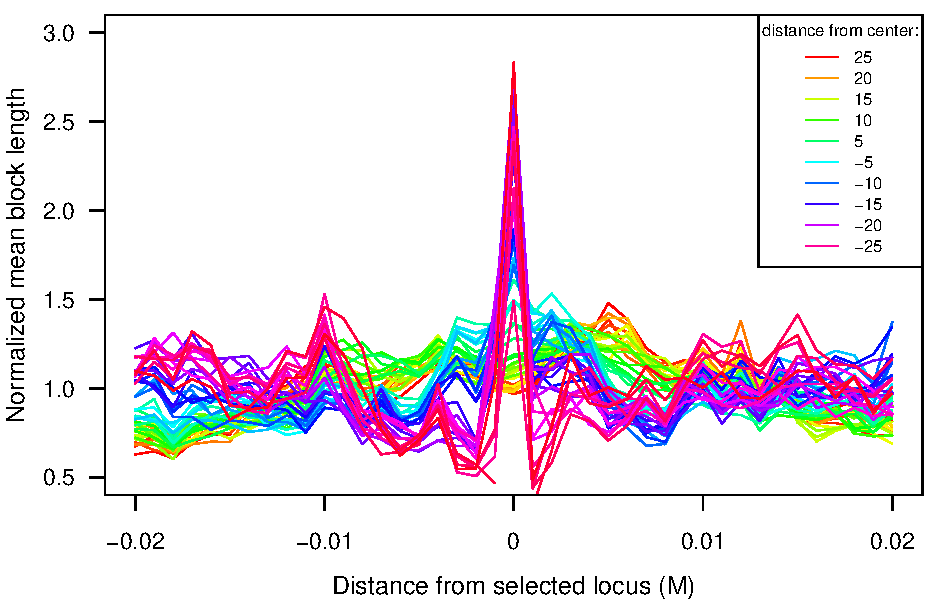
\includegraphics{figs/ratioAdjacentBlocksAlongChromAncBConditioning.pdf}
\caption{Ratio $\frac{2\sum{l_B(m_i)}}{\sum{l_A(m_i-)+I_A(m_i+)}}$ of mean block length and adjacent block lengths across a simulated chromosome with a single underdominant site and conditioning on ancestry $B$ at the selected site ($s=0.01, T=1000$).  Each line represents a deme and is normalized by mean block length across the chromosome in the deme.}\label{Supp:ratioBlockAdjacent}
\end{figure}


\begin{figure}
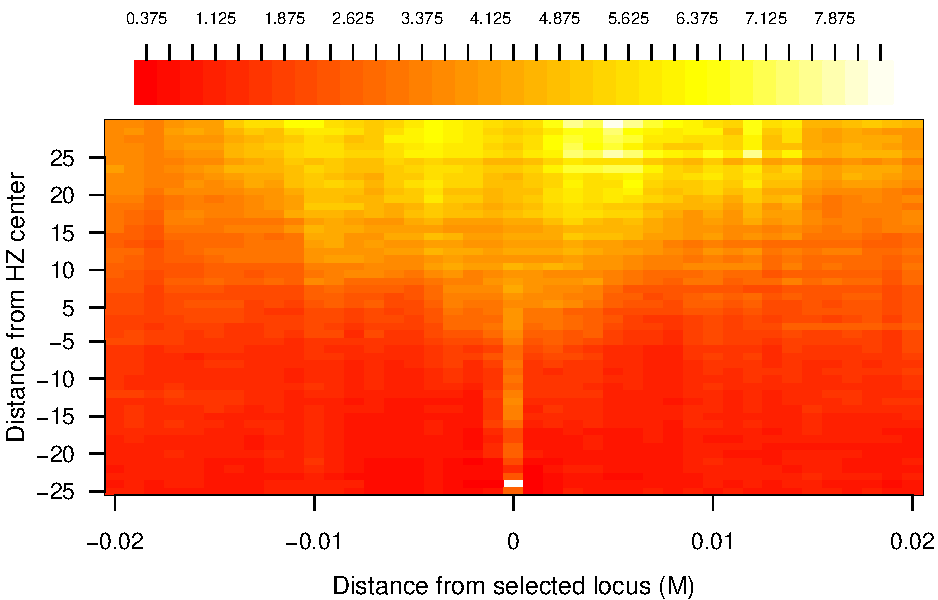
\includegraphics{figs/ratioAdjacentBlocksAlongChromHeatmapAncBConditioning.pdf}
\caption{Heatmap of $\frac{2\sum{l_B(m_i)}}{\sum{l_A(m_i-)+I_A(m_i+)}}$ across a simulated chromosome with a single underdominant site and conditioning on ancestry $B$ at the selected site ($s=0.01, T=1000$). }\label{Supp:ratioBlockAdjacentHeatmap}
\end{figure}


\begin{figure}
    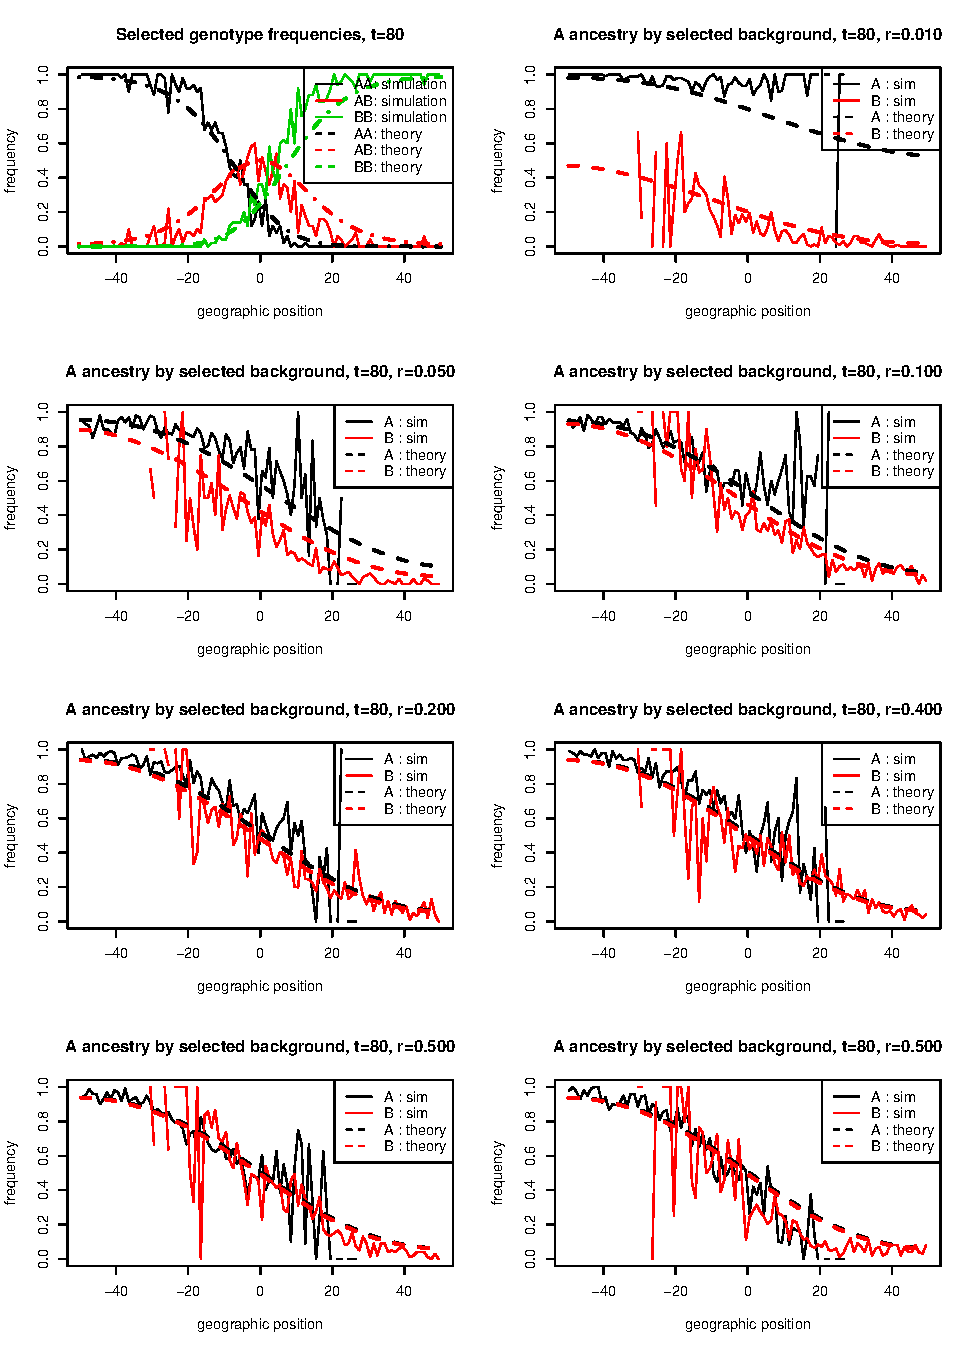
\includegraphics[height=0.8\textheight]{figs/cond_freqs_comparison_tau_80.pdf}
    \caption{
        \textbf{Conditional frequencies of ancestry $A$ at $\tau=80$},
        comparing simulation and theory, with $\sigma=3$ deme spacings, $s=0.05$, and 50 individuals per deme.
        The top left figure shows observed and expected genotype frequencies for the two homozygotes and the heterozygote at the selected locus;
        expected genotype counts were obtained assuming random mating,
        and by solving equation \eqref{eqn:cline_pde} numerically.
        The remaining figures show observed and expected frequencies of $A$ ancestry,
        separately conditioned on the identity of the linked allele at the selected site.
        Observed frequencies become much noisier where the linked allele becomes rarer.
    } \label{sfig:condAlleleFreq_tau80_comparison}
\end{figure}


\begin{figure}
    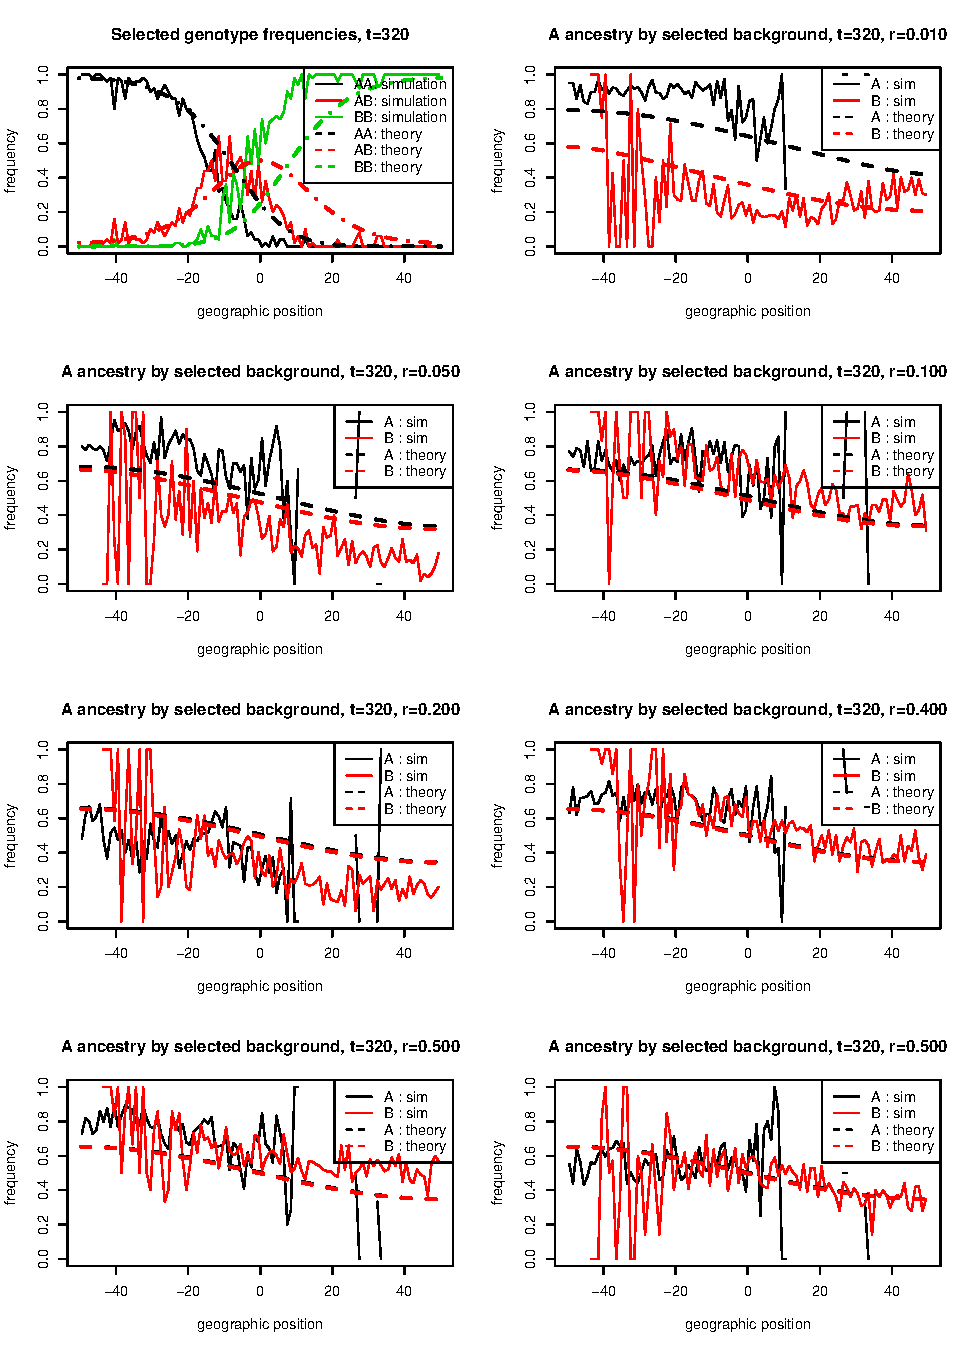
\includegraphics{figs/cond_freqs_comparison_tau_320.pdf}
    \caption{
        \textbf{Conditional frequencies of ancestry $A$ at $\tau=320$},
        as in figure \ref{sfig:condAlleleFreq_tau80_comparison}.
        Deviations are larger than at $\tau=80$, 
        due to genetic drift.
    } \label{sfig:condAlleleFreq_tau320_comparison}
\end{figure}


\begin{figure}
    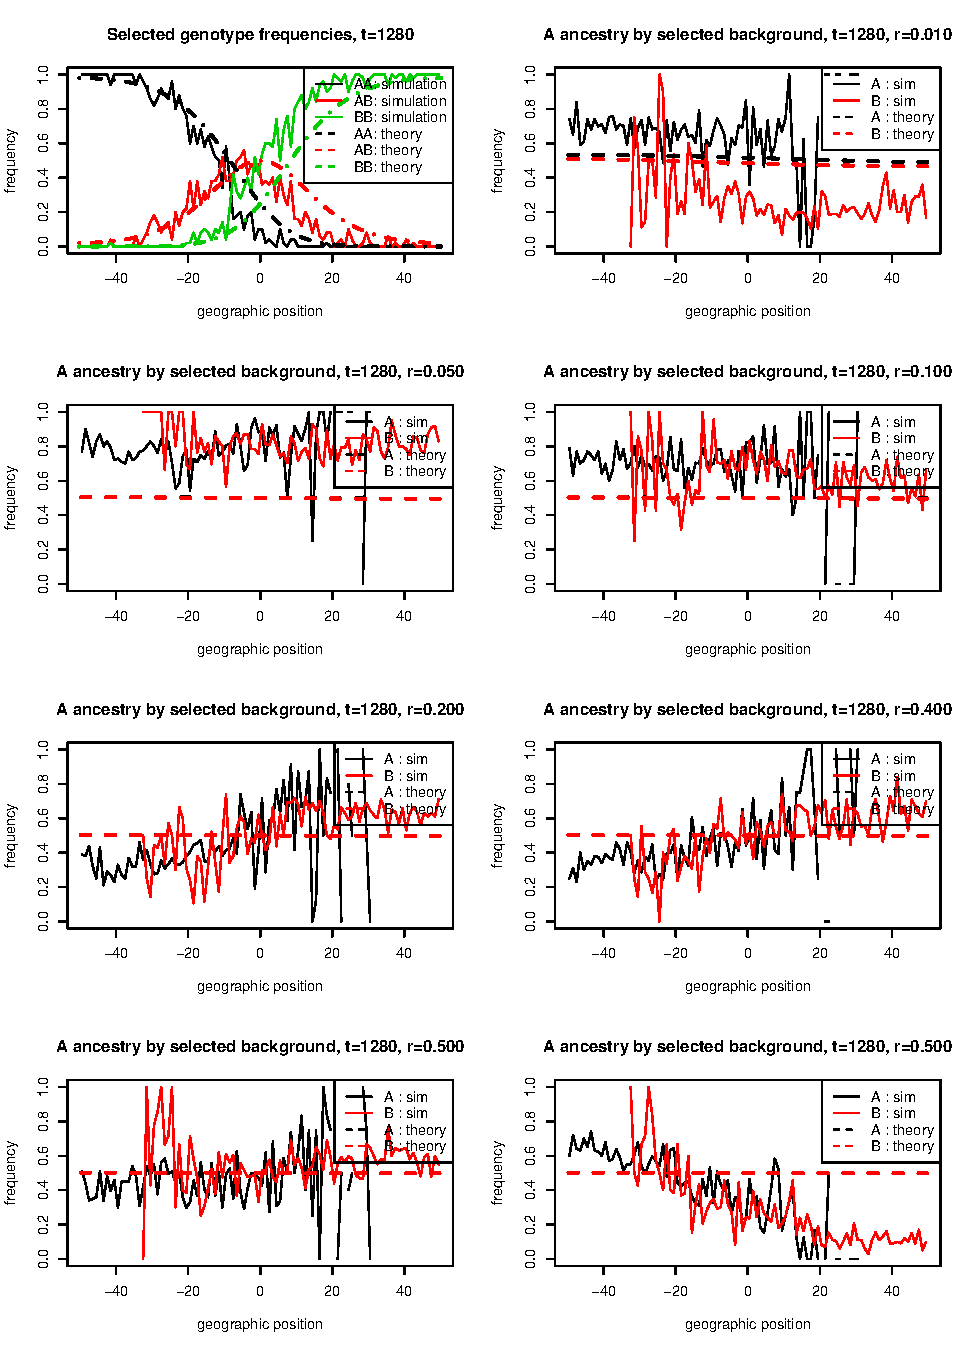
\includegraphics{figs/cond_freqs_comparison_tau_1280.pdf}
    \caption{
        \textbf{Conditional frequencies of ancestry $A$ at $\tau=1280$},
        as in figure \ref{sfig:condAlleleFreq_tau80_comparison}.
        Deviations are larger still than at $\tau=320$, 
        due to genetic drift.
    } \label{sfig:condAlleleFreq_tau1280_comparison}
\end{figure}

\begin{figure}
    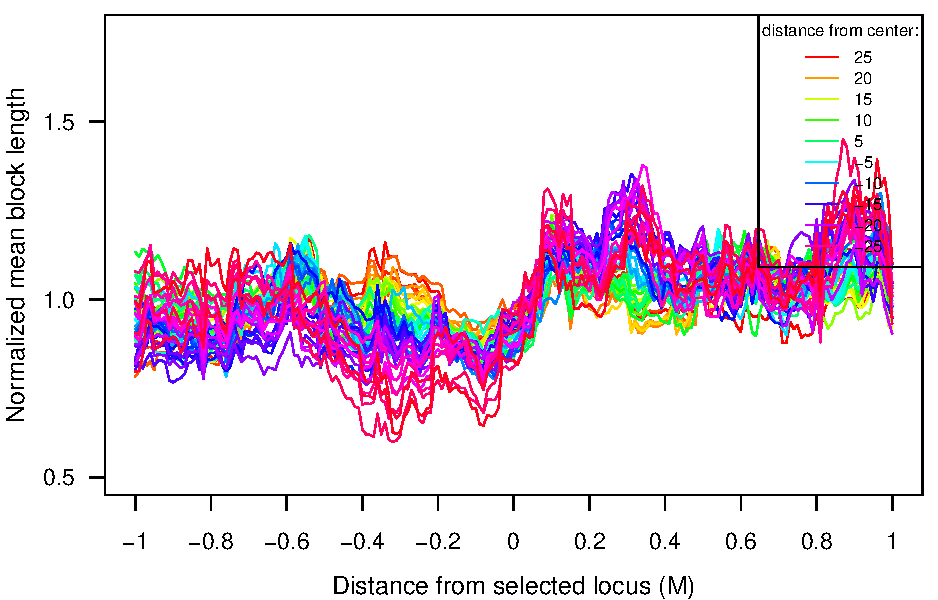
\includegraphics{figs/s001_adjacentBlocksAlongChromAncBConditioning}
    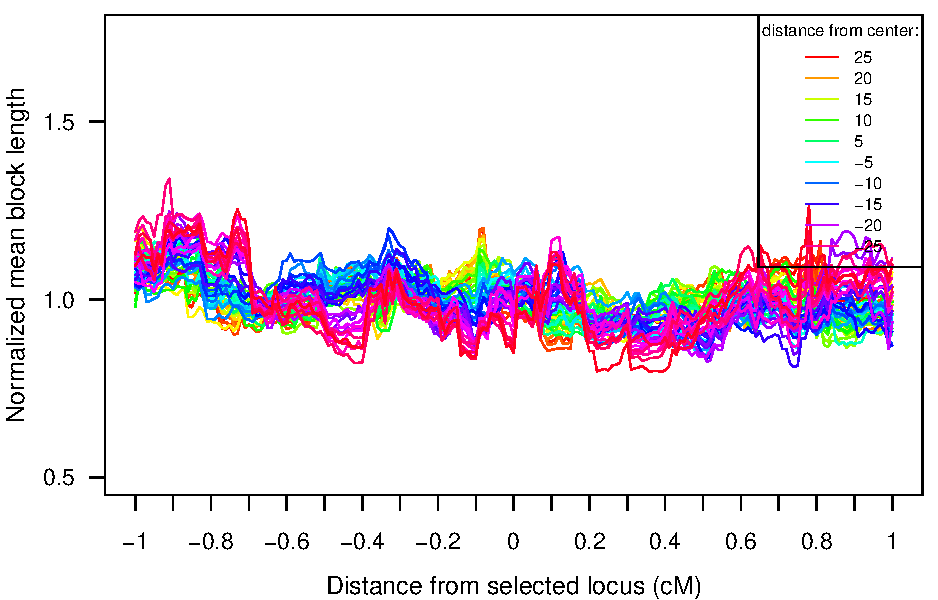
\includegraphics{figs/s001_adjacentBlocksAlongChromNoConditioningHighRes}
        \caption{
     Block lengths along chromosome under $s=0.001$, conditioning on ancestry B (upper) and without conditioning (lower) alisa{is this perhaps an instance where we would need to have more demes to see a signal?
    }
    } \label{sfig:blockLengthPlot_t1000_s0.001}
\end{figure}




% \end{document}
